Per l'esecuzione del'esperienza è stato utilizzato il seguente apparato sperimentale:
\begin{itemize}
	\item Un calorimetro di Regnault con coperchio munito di due resistori e un agitatore;
	\item Un termometro digitale;
	\item Un generatore di tensione continua;
	\item Un multimetro impostato come voltmetro;
	\item Un multimetro impostato come amperometro;
	\item Un cronometro digitale;
	\item Una bilancia digitale.
\end{itemize}

\begin{table}[H]
	\centering
	\begin{tabular}{|c|c|}
		\hline
		\textbf{Strumenti di misura} & \textbf{Risoluzione} \\
		\hline
		Termometro digitale & $0.1\ ^{\circ}C$ \\
		\hline
		Cronometro digitale & $0.01\ s$ \\
		\hline
		Bilancia digitale & $0.01\ g$ \\
		\hline
	\end{tabular}
	\caption{Risoluzione degli strumenti di misura utilizzati}
	\label{tab:}
\end{table}

\begin{figure}[H]
	\centering
	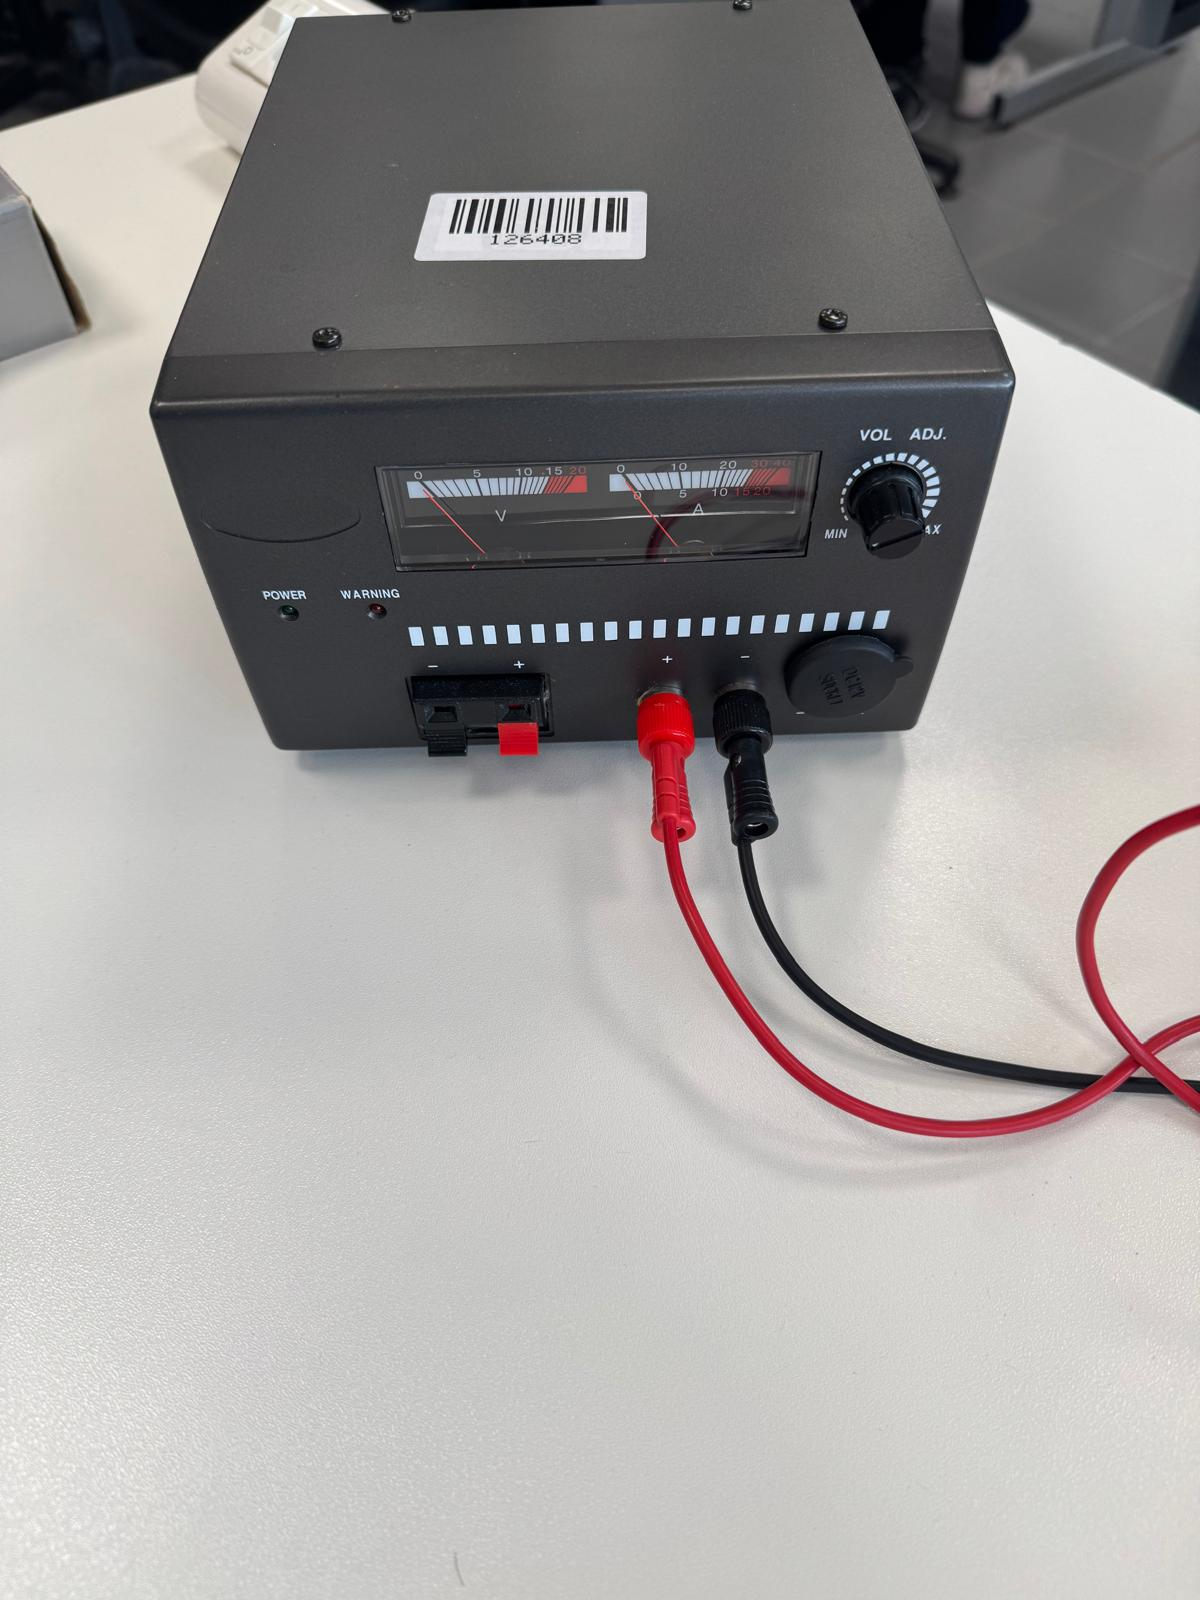
\includegraphics[width=0.35\textwidth]{./figures/generatore}
	\caption{Generatore di tensione continua utilizzato per l'esperimento.}
\end{figure}

\begin{figure}[H]
	\centering
	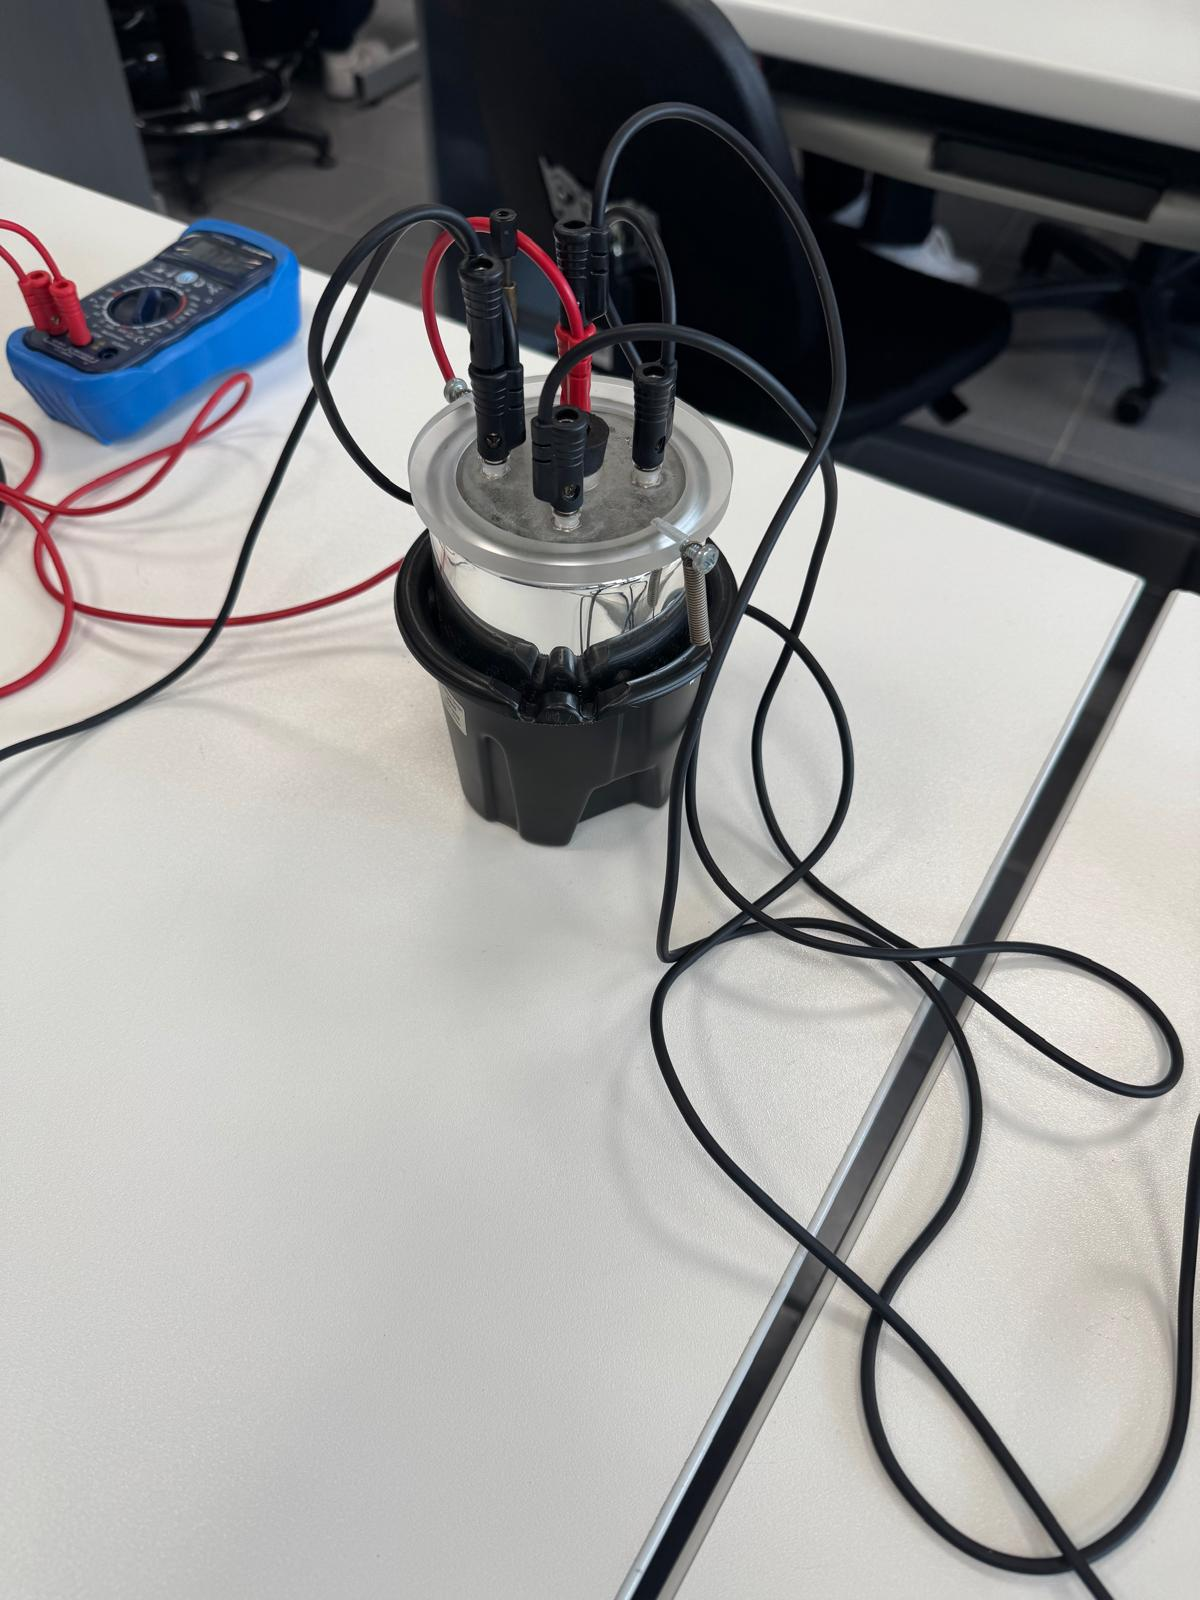
\includegraphics[width=0.4\textwidth]{./figures/calorimetro}
	\caption{Circuito assemblato per l'esecuzione dell'esperimento.}
\end{figure}

